\documentclass{aims}

%%%%%%%%%%%%%%%%%%%%%%%%%%%%%%%%%%%%%%%%%%
\usepackage{txfonts}
\usepackage{booktabs}
\usepackage{longtable}
\usepackage{lipsum}
\usepackage{hyperref}
\hypersetup{colorlinks=true}
\usepackage{subcaption}
\usepackage{placeins}
\usepackage{tikz}
\usetikzlibrary{automata,positioning,arrows}

%%%%%%%%%%%%%%%%%%%%%%%%%%%%%%%%%%%%%%%%%%
\usepackage[backend=bibtex,sorting=none]{biblatex}
\addbibresource{./references/paper.bib}
\addbibresource{./references/unsorted.bib}
\addbibresource{./references/def_model.bib}
\addbibresource{./references/comp_etym.bib}

%%%%%%%%%%%%%%%%%%%%%%%%%%%%%%%%%%%%%%%%%%
\newcommand{\ep}{\varepsilon}
\newcommand{\eps}[1]{{#1}_{\varepsilon}}

\def\typeofarticle{Research Article} \def\currentvolume{1} \def\currentissue{1}
\def\currentyear{2021} \def\currentmonth{} \def\ppages{1--30} \def\DOI{to
appear} \def\Received{June 2022} \def\Accepted{July 2022} \def\Published{October
2022 }
\numberwithin{equation}{section}
\DeclareMathOperator*{\essinf}{ess\,inf}

\usepackage{array}
\newcolumntype{L}{>{\arraybackslash}m{8cm}}

%%%%%%%%%%%%%%%%%%%%%%%%%%%%%%%%%%%%%%%%%%
\begin{document}

\title{Survey on Definition Modeling}

\author{%
    Noah Gardner\affil{1},
    Hafiz Khan\affil{2},
    Chih-Cheng Hung\affil{1}\corrauth
}%

% \shortauthors is used in copyright information in the end of the paper
\shortauthors{the Author(s)}

\address{%
    \addr{\affilnum{1}}{Laboratory of Machine Vision and Security Research, %
        College of Computing and Software Engineering, Kennesaw State %
        University, Marietta GA, USA}%
    \addr{\affilnum{2}}{Laboratory of Ubiquitous Data Mining, %
        College of Computing and Software Engineering, Kennesaw State %
        University, Marietta GA, USA}}
\corraddr{chung1@kennesaw.edu}

\begin{abstract}
    Definition modeling, the task of generating a definition for a given term,
    is a relatively new area of research applied in the evaluation of word
    embeddings that is gathering attention. Automatic generation of dictionary
    quality definitions has many applications in natural language processing,
    such as sentiment analysis, machine translation, and word sense
    disambiguation. Additionally, definition modeling is also useful for
    evaluating the quality of word embeddings. As more research is done in this
    field, the need for a summary of different applications, approaches, and
    obstacles grows apparent. This survey aims to provide an overview of the
    current research in definition modeling, and to provide a list of future
    directions and trends.
\end{abstract}
\keywords{Definition modeling; definition generation}
\maketitle

\section{Introduction}
Definitions are explicit representations of words or phrases that are valuable
for exposing the aspects of a given term. In general, definitions are
unambiguous and succinct: they should be easy to read and understand. Recent research
has allowed the creation of neural language models that can generate useful
definitions from embeddings \cite{bosc_auto_2018, hill_learning_2016, washio_bridging_2019}. Word embeddings are vector representations of words that have been employed in a variety of \textit{natural language
    processing} (NLP) tasks. They are useful for capturing lexical syntax and
semantic similarity. Mikolov et al. \cite{mikolov_distributed_2013} have shown that
basic mathematical operations applied to word embeddings can have meaningful
language understanding. However, as continuous representations, the
interpretability of word embeddings is limited.

\begin{figure}[h]
    \centering
    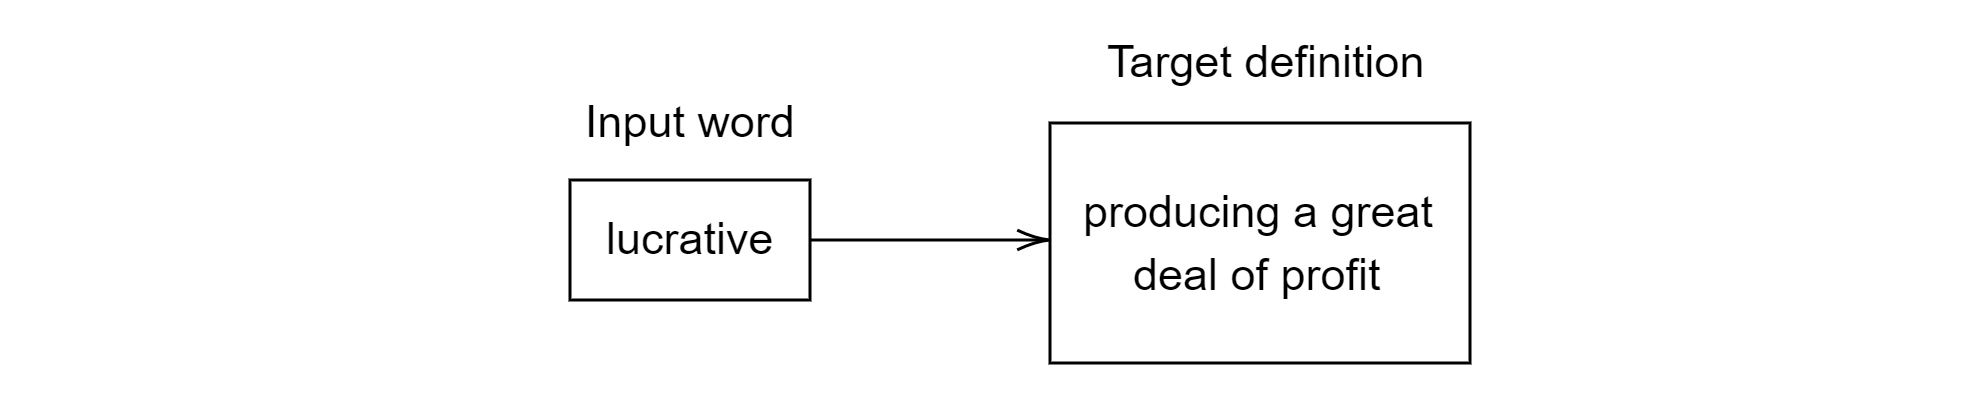
\includegraphics[width=.9\textwidth]{assets/figures/monoseme.png}
    \caption{Monoseme example word and definition. A definition model could
        generate the definition \textit{producing a great deal of profit} for the
        input word \textit{lucrative}.}
    \label{fig:monoseme}
\end{figure}

The problem of \textit{definition modeling} was proposed by Noraset et al.~\cite{noraset_definition_2016} to evaluate word embeddings. The task of definition modeling is to generate a definition for a given term. The goal of a model trained on this task is to train on word embedding and definition pairs to learn to generate a definition for a given word or phrase. An example of a \textit{monoseme} (word with a single definition) is given in Figure~\ref{fig:monoseme}. Given the input word \textit{lucrative}, a model trained on
the task of definition modeling would produce the output definition
\textit{producing a great deal of profit}.

\begin{figure}[h]
    \centering
    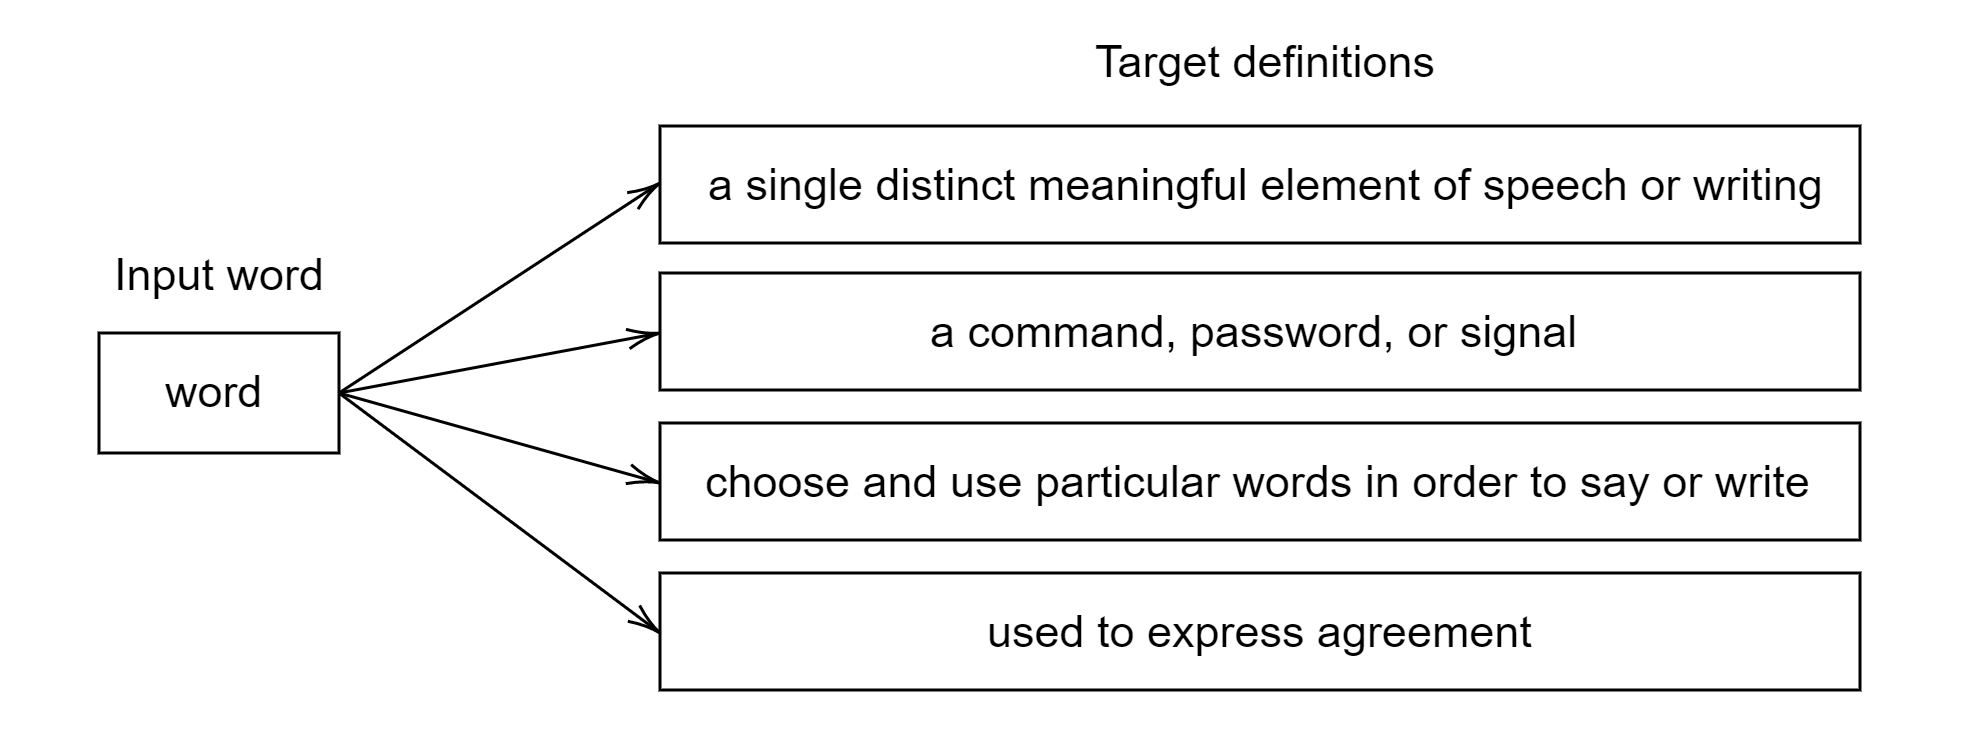
\includegraphics[width=.9\textwidth]{assets/figures/polyseme.png}
    \caption{Polyseme example word and definition. A definition model could generate any of the target definitions.}
    \label{fig:polyseme}
\end{figure}

In addition to being a relatively new language modeling task, definition
modeling has attracted attention from the literature in a number of areas.
First, it was shown that the definition model has poor performance when
generating definitions for polysemes: words with multiple definitions
\cite{gadetsky_conditional_2018}. An example polysemous word is shown in Figure
\ref{fig:polyseme}. Given the input \textit{word}, the goal of a definition
model would be to generate one of the target definitions, most ideally the
closest definition to the word sense of the input. However, it is challenging to
know the word sense given only the input word.

The problem of polysemous words was not addressed in the original work, as only one definition mapped to each word. Once researchers attempted to address this problem, they found that the definition model could not learn the semantics of the polyseme with only the word as an input. Therefore, it was necessary to augment the definition model with additional information, namely, an example sentence that sets the word to be defined (\textit{definiendum}) inside to
provide context. This method has been shown to alleviate the problem of generating definitions for polysemes and also improve the performance of the definition model on several measures~\cite{bevilacqua_generationary_2020,
    gadetsky_conditional_2018, mickus_mark_2019}.

\begin{figure}[h]
    \centering
    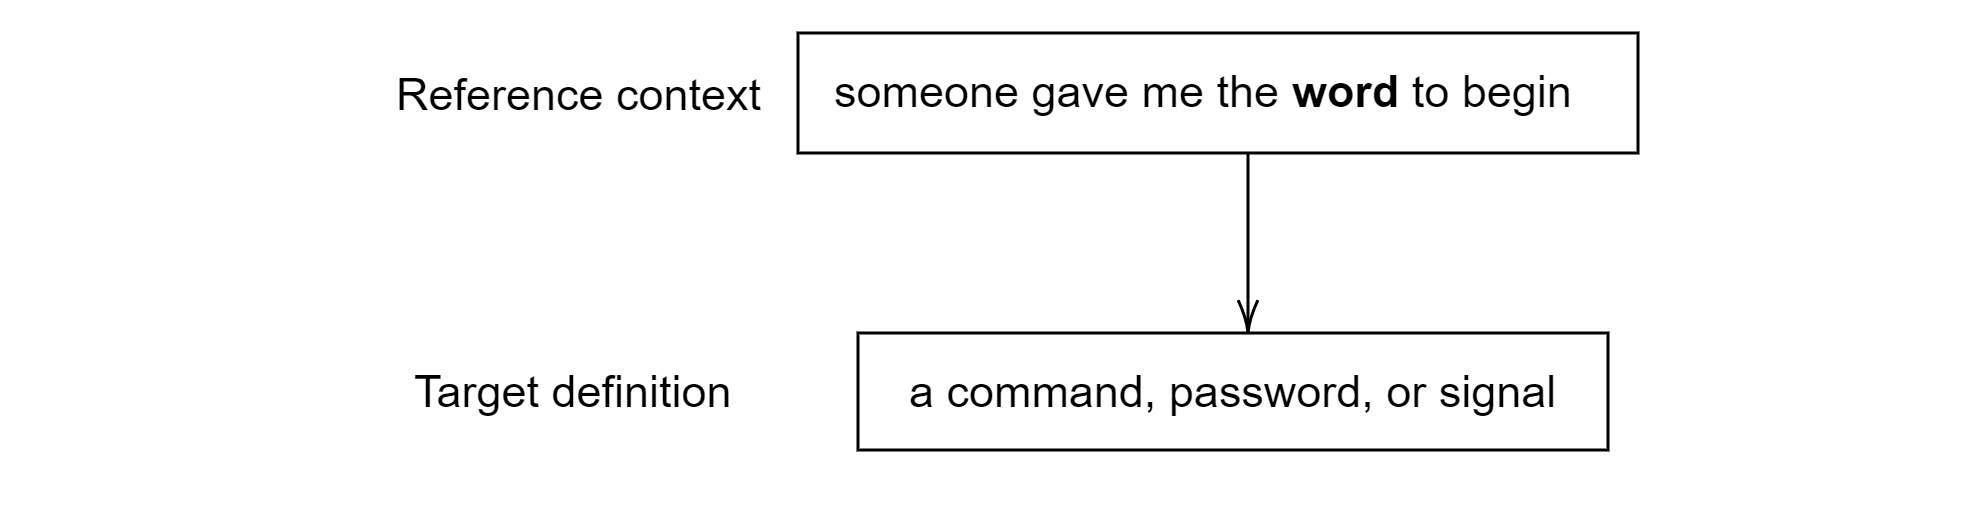
\includegraphics[width=.9\textwidth]{assets/figures/context.png}
    \caption{Context-dependent definition task. The word to be defined is marked
        in bold. In this case, although \textbf{word} is a polyseme, there is only
        one correct target definition due to the contextual information provided.}
    \label{fig:context_poly}
\end{figure}

Definition modeling, especially as a sequence-to-sequence task, is similar to other NLP tasks, such as \textit{word-sense disambiguation}, \textit{word-in-context}, and \textit{definition extraction}~\cite{bevilacqua_generationary_2020, huang_cdm_2021}. When using context to generate a definition from an input word, the input's word sense must be extracted to select the correct definition. The goal of word-sense disambiguation is similar in that the goal of word-sense disambiguation is to identify the sense of a word used in a sentence. Similarly, definition extraction seeks to extract definitions of terms from an existing corpus~\cite{huang_cdm_2021}. Figure~\ref{fig:context_poly} shows an example of definition modeling in a context-dependent situation. In the example, a reference context is given. Inside the reference context, a target word
\textit{word} is marked as the word to be defined. The goal of a definition model given this context and marked word would be to generate the target definition \textit{a command, password, or signal}.

Our paper is organized into three sections. Section 2 reviews definition modeling methods as well as word embeddings. Section 3 shares benchmark datasets
and statistics that can be used when formulating and evaluating a definition modeling method. Section 4 explores challenges encountered in this research field and gives suggestions for future work.

\section{Methodologies Explored}
main key points -- definition generation and word embedding (similarity disabmiguity etc. polysemy). Few line of text should be here.  

\begin{longtable}{|p{3.5cm}|p{3.5cm}|p{3.5cm}|p{3.5cm}|}
    \caption{Definition Modeling Methods}                                                                                                                                                                                                                                                                                                                                                   \\
    \hline
    Article                                                                                                                   & Evaluation                                                       & Dataset                                                                                                                                       & Models                                   \\
    \hline
    \citeauthor*{noraset_definition_2016} \citeyear{noraset_definition_2016} \cite{noraset_definition_2016}                   & Perplexity, BLEU                                                 & GCIDE, Custom                                                                                                                                 & RNN, Word2Vec, LSTM                      \\
    \hline
    \citeauthor*{gadetsky_conditional_2018} \citeyear{gadetsky_conditional_2018} \cite{gadetsky_conditional_2018}             & Perplexity, BLEU                                                 & Oxford                                                                                                                                        & LSTM, Word2Vec, SkipGram                 \\
    \hline
    \citeauthor*{chang_what_2019} \citeyear{chang_what_2019} \cite{chang_what_2019}                                           & Precision, ROUGE-L, Cosine similarity                            & Oxford                                                                                                                                        & ELMo, BERT, FastText                     \\
    \hline
    \citeauthor*{washio_bridging_2019} \citeyear{washio_bridging_2019} \cite{washio_bridging_2019}                            & Perplexity, BLEU                                                 & \cite{noraset_definition_2016}, \cite{gadetsky_conditional_2018}                                                                              & Encoder/decoder                          \\
    \hline
    \citeauthor*{mickus_mark_2019} \citeyear{mickus_mark_2019} \cite{mickus_mark_2019}                                        & Perplexity                                                       & \cite{noraset_definition_2016}, \cite{gadetsky_conditional_2018}, Custom                                                                      & GloVe, Transformer, sequence-to-sequence \\
    \hline
    \citeauthor*{li_explicit_2020} \citeyear{li_explicit_2020} \cite{li_explicit_2020}                                        & BLEU, METEOR, Human                                              & WordNet, Oxford                                                                                                                               & CNN, LSTM                                \\
    \hline
    \citeauthor*{bevilacqua_generationary_2020} \citeyear{bevilacqua_generationary_2020} \cite{bevilacqua_generationary_2020} & Perplexity, BLEU, ROUGE-L, METEOR, BERTScore                     & Oxford \cite{chang_what_2019}, Sem-Cor \cite{miller_semantic_1993}, Wiktionary, GCIDE \cite{noraset_definition_2016}, Hei++ (Custom), WordNet & BART                                     \\
    \hline
    \citeauthor*{sojka_evaluating_2020} \citeyear{sojka_evaluating_2020} \cite{sojka_evaluating_2020}                         & BLEU, rBLEU (recall-based), fBLEU (harmonic mean of BLEU, rBLEU) & Wiktionary, OmegaWiki, WordNet                                                                                                                & AdaGram, Word2Vec, CNN, RNN              \\
    \hline
    \citeauthor*{huang_cdm_2021} \citeyear{huang_cdm_2021} \cite{huang_cdm_2021}                                              & BLEU, ROUGE-L, METEOR, BERTScore                                 & Wikipedia                                                                                                                                     & BERT                                     \\
    \hline
    \citeauthor*{reid_vcdm_2020} \citeyear{reid_vcdm_2020} \cite{reid_vcdm_2020}                                              & BLEU, BERTScore (Precision, Recall, F1), Human                   & Oxford, Urban, Wikipedia, Cambridge, Robert (French)                                                                                          & BERT, LSTM                               \\
    \hline
    % \citeauthor*{noraset_definition_2016} \citeyear{noraset_definition_2016} \cite{noraset_definition_2016}                   & Perplexity, BLEU                             & GCIDE, Custom                                                                                                                                 & RNN, Word2Vec, LSTM                      \\
\end{longtable}

\subsection{Language Models}
A definition model is a language model that is trained on a set of definitions
\cite{noraset_definition_2016}. The goal of a definition model is to learn to
generate a definition ($\textbf{d} = [d_1, ..., d_T]$) for a given term $w$. The
probability of generating the $t$-th word in a definition depends on both the
previous words in the definition and the word to be defined (Eq.
\ref{eq:definition_model}).

\begin{equation}
    \label{eq:definition_model}
    p(\textbf{d} | w) = \prod_{t=1}^{T} p(d_t | d_1,...,d_{t-1}, w)
\end{equation}

Noraset et al. condition an RNN to generate a defintion from an input seed word.
They modify the model by updating the output of the recurrent unit with an
update function inspired by GRU update gate \cite{noraset_definition_2016}. They
apply pretrained word embeddings generated from Word2Vec.

In later work, it was shown that the definition model does not generate
definitions for words with ambigious word sense, especially polysemantic words.
The following context-aware definition model was proposed by
\citeauthor*{gadetsky_conditional_2018} in order to tackle this challenge
\cite{gadetsky_conditional_2018}. They extend Equation \ref{eq:definition_model}
by adding a context term ($\textbf{c} = [c_1, ..., c_T]$) which is a context or
example sentence to be used in the generation of the definition.

\begin{equation}
    \label{eq:context_aware_definition_model}
    p(\textbf{d} | w, \textbf{c}) = \prod_{t=1}^{T} p(d_t | d_1,...,d_{t-1}, w, \textbf{c})
\end{equation}

In order to generate a definition, they use an attention-based SkipGram model to
extract dimensions from the embedding which contain the most relevant
information.

\cite{huang_cdm_2021} focused on language generation, etc.\cite{gadetsky_conditional_2018} conditional generation of definition.\cite{zheng_decompose_2021}, chienese defition generation.
\cite{sojka_evaluating_2020}, generation
\cite{li_explicit_2020}
\cite{bevilacqua_generationary_2020}
\cite{zhang_improving_2020}
\cite{yang_incorporating_2020}
\cite{ishiwatari_learning_2019}a general task of defining un-
known phrases given their contexts.

\subsection{Word Embedding}
In recent years, definition modeling has gained popularity, and researchers proposed various methods to map between definition and the target word. One of the significant issues in mapping words with the dictionary is contextual ambiguity and embedding-based word representation. In NLP, word embedding represents the vector representation of words that encodes the word's meaning such that similar words have similar vector space. There are various word embedding techniques used to resolve ambiguity between words. In the definition modeling problem, word to vector representation is a key factor in modeling definition words/terms for a given term. 

\cite{bosc_auto_2018} exploited dictionary recursivity into consideration and proposed an autoencoder-based word embedding algorithm, and generated a single embedding per word—the proposed auto-encoder model comprises of LSTM encoder and decoder. The authors introduced three embeddings - i) definition embeddings produced by the proposed definition encoder, ii) input embeddings for the encoder, and iii) output embeddings. While modeling these embedding models, the author incorporates consistency penalty as soft weight in their cost function to enforce input embedding and definition embedding closer. 

In \cite{washio_bridging_2019}, the authors consider lexical-semantic relations between the defined word and defining words using unsupervised methods to propose definition modeling. To learn embedding author proposed LSTM based encoder and decoder with additional cost function to learn word-pair embeddings in the decoder and capture lexical-semantic relations.

Dictionary embeddings often follow a genus + differentia structure for a dictionary definition~\cite{noraset_definition_2016}—author capture hypernyms embedding following proper genus database WebIsA containing hypernym relations. In addition, the author incorporates char-CNN to capture affixes to model gated-RNN based definition modeling.


Word-embeddings are learned from large corpora. Therefore, it may consists of biases such as gender, race, religion, etc. On the otherhand, word dictionaries contain unbiased, concise definitions. To overcome these biases by utilizing pre-trained word-embedding, authors learned embedding from existing input word embeddings using encoder-decoder architecture by defining decoder cost function that considers dictionary agreement as a constraint and decoded the debiased embedding~\cite{kaneko_dictionary_2021}. 

% \subsection{Methodology Comparisons}
% Mostly focus on different group of papers focused on similar task with similar
% datasets. show tables that mentioned - dataset names, algorithm used
% (highlevel), performances (acc, f1 or so on). Need to think after writing those
% previous sections.

% \subsection{Deep Learning}
% general diagram for deep learning approach.


% Semi-supervised approach \cite{patra_bilingual_2019}.

% \cite{wu_2021_sequence}We computationally model the processes of
% word borrowing from a donor word to an incorporated
% word, and vice versa, by answering
% two questions: (1) what does a word look
% like incorporated into another language, and
% in the opposite direction (2) where did a word
% come from? We experiment with several
% model variants, including LSTM encoderdecoders,
% copy attention, and Transformers.

% \cite{wu_computational_2020} For our model, we used a LSTM with an embedding
% dimension of 128 and hidden dimension of 128.
% The output of the last hidden state is passed to a fully connected layer with a sigmoid activation function.

% \subsubsection{Parameters and Evaluation}
% \begin{itemize}
%     \item Perplexity
%     \item Precision
%     \item BLEU score
%     \item ROUGE-L
%     \item Cosine similarity
% \end{itemize}

% In general, the performance of generative definition models are evaluated using
% perplexity and BLEU score.

\section{Datasets and analysis}
\begin{table}
    \centering
    \caption{Datasets used in definition modeling}
    \begin{tabular}{|ll|}
        \hline
        Dataset          & Methods                              \\
        \hline
        Oxford & \cite{bevilacqua_generationary_2020,
        chang_what_2019,
        gadetsky_conditional_2018,
        ishiwatari_learning_2019,
        li_explicit_2020,
        mickus_mark_2019,
        reid_vcdm_2020,
        washio_bridging_2019} \\
        WordNet & \cite{bevilacqua_generationary_2020,
        ishiwatari_learning_2019,
        kabiri_evaluating_2020,
        li_explicit_2020,
        mickus_mark_2019,
        noraset_definition_2016,
        washio_bridging_2019} \\
        Urban Dictionary & \cite{reid_vcdm_2020,
        ishiwatari_learning_2019,
        ni_learning_2017}\\
        Wikipedia & \cite{huang_cdm_2021,
        reid_vcdm_2020}\\
        Wiktionary & \cite{bevilacqua_generationary_2020,
        kabiri_evaluating_2020}\\
        OmegaWiki & \cite{kabiri_evaluating_2020}\\
        Hei++ & \cite{bevilacqua_generationary_2020}\\
        \hline
    \end{tabular}
    \label{tab:eval}
\end{table}

Various benchmark datasets have been proposed for the training and evaluation of
definition models. In this section, we provide brief descriptions of each
dataset and provide analysis of various characteristics of the datasets.

\textbf{Oxford Dictionary:}
\textit{The Oxford Dictionary of
    English}\footnote{\href{https://languages.oup.com/}{https://languages.oup.com/}}
is a free dictionary of English words and phrases. Collected by Gadetsky et
al., this dataset features contextual information for each word along with
the definition \cite{gadetsky_conditional_2018}. This dataset is useful for
evaluating the ability of a model to generate definitions for polysemous
words.

\textbf{GCIDE/WordNet:}
\textit{The GNU Collaborative International Dictionary of
    English}\footnote{\href{https://gcide.gnu.org.ua/}{https://gcide.gnu.org.ua/}}
(GCIDE) is a free dictionary supplemented with some definitions from
WordNet\footnote{\href{https://wordnet.princeton.edu/}{https://wordnet.princeton.edu/}}.
Available under the GNU General Public License, GCIDE is a useful corpus for
dictionary definitions for general words. This dataset was modified by
Noraset et al. for their original definition model
\cite{noraset_definition_2016}. Kabiri et al. also provide a modified
dataset for their method \cite{kabiri_evaluating_2020}.

\textbf{Urban Dictionary:}
\textit{The Urban
    Dictionary}\footnote{\href{https://www.urbandictionary.com/}{https://www.urbandictionary.com/}}
is a free dictionary of slang words and phrases where definitions are
crowd-sourced by users. Proposed by Ni et al., the Urban Dictionary dataset
is useful for idioms and rarely-used phrases which are not contained in
other dictionary datasets due to only containing slang definitions
\cite{ni_learning_2017}.

\textbf{Wikipedia:}
\textit{The English
    Wikipedia}\footnote{\href{https://en.wikipedia.org/}{https://en.wikipedia.org/}}
is a free online encyclopedia. Collected by Ishiwatari et al., it combines
the useful tasks of WordNet, Oxford Dictionary, and Urban Dictionary, since
it contains descriptions of many concepts along with context to be used in
context-aware models \cite{ishiwatari_learning_2019}.

\textbf{Wiktionary:}
\textit{Wiktionary}\footnote{\href{https://en.wiktionary.org/}{https://en.wiktionary.org/}}
is a free online dictionary from the same parent organization as Wikipedia
(Wikimedia Foundation). It is useful as it provides a definitions for a large
number of languages which can allow for multi-lingual definition modeling. We
share statistics for the English version of Wiktionary, since most definition
modeling methods focus on English.

\textbf{OmegaWiki:}
Similar to Wiktionary, \textit{OmegaWiki} is a multi-lingual dictionary. The
goal of OmegaWiki is to create a lexical resource with all definitions of all
words in every language. Kabiri et al. use this resource due to the availability
of a variety of languages \cite{kabiri_evaluating_2020}.

\textbf{Hei++:}
\textit{Hei++}\footnote{\href{http://generationary.org/}{http://generationary.org/}}
is a unique evaluation dataset proposed by Bevilacqua et al.
\cite{bevilacqua_generationary_2020}. Rather than contain singular words or
phrases to define like the other dictionary-based resources, this dataset is
comprised of adjective-noun phrases. An example phrase, \textit{starry sky}, can
be defined as 'The sky as it appears at night, especially when lit by stars'.
This is a hand-made dataset which was create with the assistance of an expert
lexicographer. As a result, this dataset is small and should be used in model
evaluation rather than training. Our dataset analysis shows no overlap of this
dataset with the other benchmark datasets, implying this dataset can also be
used to evaluating the ability of a model to generalize on never-before-seen
data.

\subsection{Definition Statistics}

In our analysis of the datasets above, to distinguish the benchmark datasets
provided by the correlating authors, we use the notations listed in Table
\ref{tab:ds_notations}.

\begin{table}[h]
    \centering
    \caption{Dataset notations}
    \begin{tabular}{|l|l|}
    \hline
    Dataset                  & Description                                                                                     \\
    \hline
    \textit{wordnet-nor}     & WordNet dataset, from Noraset et al. \cite{noraset_definition_2016}                             \\
    \textit{urban-ni}        & Urban Dictionary dataset, from Ni et al. \cite{ni_learning_2017}                                \\
    \textit{oxford-gad}      & The Oxford Dictionary of English dataset, from Gadetsky et al. \cite{gadetsky_conditional_2018} \\
    \textit{wordnet-ish}     & WordNet dataset, from Ishiwatari et al. \cite{ishiwatari_learning_2019}                         \\
    \textit{wikipedia-ish}   & Wikipedia dataset, from Ishiwatari et al. \cite{ishiwatari_learning_2019}                       \\
    \textit{wikitionary-kab} & Wikitonary English dataset, from Kabiri et al. \cite{kabiri_evaluating_2020}                    \\
    \textit{wordnet-kab}     & WordNet dataset, from Kabiri et al. \cite{kabiri_evaluating_2020}                               \\
    \textit{omega-kab}       & OmegaWiki dataset, from Kabiri et al. \cite{kabiri_evaluating_2020}                             \\
    \textit{hei++-bev}       & Hei++ dataset, from Bevilacqua et al. \cite{bevilacqua_generationary_2020}                      \\
    \hline
\end{tabular}

    \label{tab:ds_notations}
\end{table}

First, in Table \ref{tab:defs}, we provide some analysis on the definition
statistics of the datasets. We evaluate all splits (train, test, and validate)
for each dataset by combining all the words and corresponding definitions. The
table shows the number of unique words and total number of definitions for each
dataset. Of note, some datasets provide the same definition for the same word,
meant to be used in a context-aware model. In this analysis, we ignore the
context phrases and treat these duplicate definitions as independent. We also
show the mean length of the definitions, the standard deviation of the lengths,
as well as the \textit{definitions per word} (DPW).

\begin{table}
    \centering
    \caption{Definition statistics}
    \begin{tabular}{|l|rr|rrr|}
    \hline
    Dataset        & Words   & Definitions & DPW  & Mean length & SD length \\
    \hline
    wikipedia-ish  & 168,753 & 988,690     & 5.86 & 5.99        & 4.53      \\
    urban-ni       & 240,334 & 507,504     & 2.11 & 12.11       & 7.71      \\
    wordnet-nor    & 22,554  & 162,925     & 7.22 & 6.60        & 5.73      \\
    oxford-gad     & 36,767  & 122,319     & 3.33 & 11.07       & 7.01      \\
    wiktionary-kab & 17,000  & 29,426      & 1.73 & 7.65        & 6.92      \\
    wordnet-kab    & 20,000  & 28,814      & 1.44 & 10.96       & 7.28      \\
    omega-kab      & 17,000  & 22,735      & 1.34 & 14.61       & 9.83      \\
    wordnet-ish    & 9,937   & 17,410      & 1.75 & 6.64        & 3.78      \\
    hei++-bev      & 713     & 713         & 1.00 & 9.44        & 2.80      \\
    \hline
\end{tabular}

    \label{tab:defs}
\end{table}

Next, in Table \ref{tab:polys}, we show the number of polysemous words in each
dataset. As with the definition statistics, we treat exact duplicate definitions
independently, because they have different contexts. The number of polysemes is
calculated as the number of words or phrases which have more than one definition
in the dataset. We show the ratio of the number of polysemous words to the total
number of words in the dataset as a percentage. The polysemous data is also
shown in Figure \ref{fig:polys}.  It is important to evaluate the polysemous
data due to the difficulty in predicting definitions for polysemous words.

\begin{table}
    \centering
    \caption{Polyseme statistics}
    \small
\begin{tabular}{|l|rrr|}
    \hline
    Dataset    & Words   & Polysemes & Polysemes (\%) \\
    \hline
    WordNet-A  & 22,554  & 22,171    & 98             \\
    Oxford     & 36,767  & 20,563    & 56             \\
    Wikipedia  & 168,753 & 77,278    & 46             \\
    WordNet-B  & 9,937   & 4,221     & 42             \\
    Urban      & 240,334 & 74,620    & 31             \\
    Wiktionary & 17,000  & 4,634     & 27             \\
    Omega      & 17,000  & 3,412     & 20             \\
    WordNet-C  & 20,000  & 3,649     & 18             \\
    Hei++      & 713     & 0         & 0              \\
    \hline
\end{tabular}

    \label{tab:polys}
\end{table}

% \begin{figure}
%     \centering
%     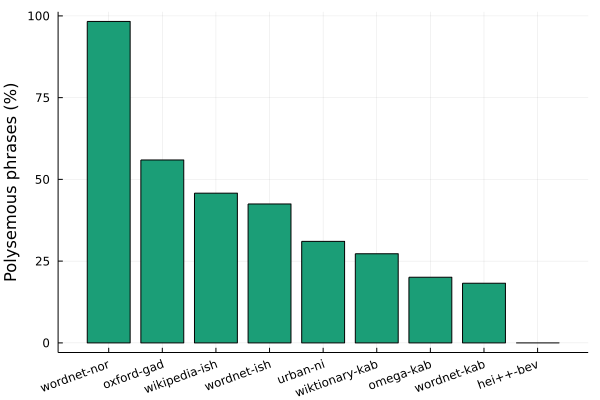
\includegraphics[width=0.65\textwidth]{assets/plots/polys_plot.png}
%     \caption{Plot of polyseme statistics, where the percentage of words or
%         phrases that are polysemous are shown.} \label{fig:polys}
% \end{figure}

Our next analysis is on the overlap present across the benchmark datasets. We
show the number of words in each dataset which are present in all other datasets
as a percentage. This allows us to identify the datasets which are most similar
and most unique. The overlap of each dataset is calculated as the unique words
that are present in each other dataset. The average overlap percentage is shown
in Figure \ref{fig:avg_overlap}, and the individual overlap of each dataset is
shown in Figure \ref{fig:overlap_all}. The Hei++ dataset is not included in the
individual overlap plot due to having an average overlap percentage of $0\%$
\cite{bevilacqua_generationary_2020}. Also, the individual overlap of each
dataset with itself is excluded, as the overlap would be $100\%$.

\begin{figure}
    \centering
    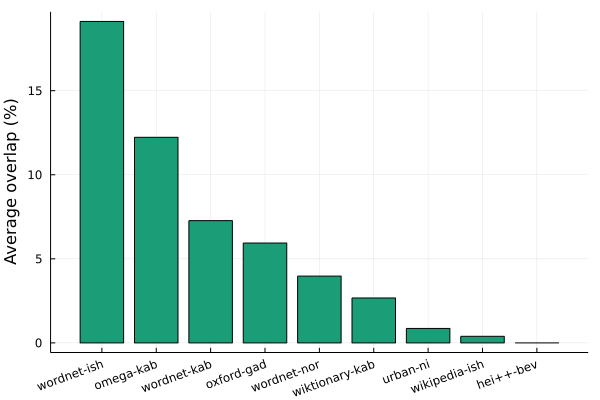
\includegraphics[width=0.7\textwidth]{assets/plots/avg_overlap.png}
    \caption{Plot of average dataset overlap.}
    \label{fig:avg_overlap}
\end{figure}

\begin{figure}
    \centering
    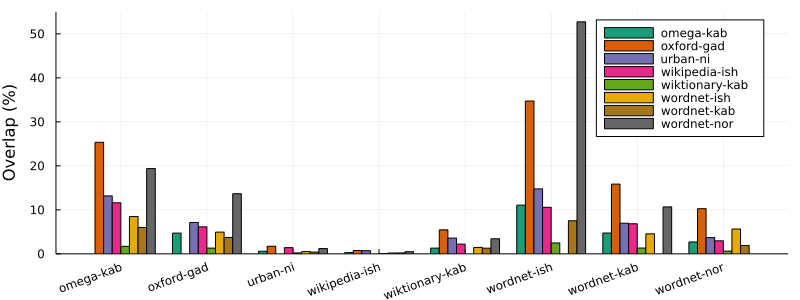
\includegraphics[width=0.95\textwidth]{assets/plots/overlap_all.png}
    \caption{Plot of individual dataset overlap.}
    \label{fig:overlap_all}
\end{figure}

\FloatBarrier
Across every benchmark dataset (excluding Hei++), a single word that is present
in each is the word \textit{movement}. Since it is the only word present in each
dataset, we show selected definitions for this word in Table \ref{tab:movement}. Several different word senses can be seen across the dataset, such as movement as something moving, a specific album, bowel movement, and even the illusion of something moving.

\begin{table}[h]
    \centering
    \caption{Definitions for the term \textit{movement}}
    \begin{tabular}{|l|l|}
    \hline
    Dataset        & Definition                                                                                                                                  \\
    \hline
    wordnet-nor    & \makecell[l]{a natural event that involves a change in the position or location of something}                                                             \\
    \hline
    oxford-gad     & \makecell[l]{a group of people with a common ideology who try together to achieve\\ certain general goals}                                                  \\
    \hline
    wordnet-ish    & a major self-contained part of a symphony or sonata                                                                                         \\
    \hline
    wikipedia-ish  & album by new order                                                                                                                          \\
    \hline
    urban-ni       & [pot credit] slang, to hit on a woman                                                                                                       \\
    \hline
    wordnet-kab    & \makecell[l]{an optical illusion of motion produced by viewing a rapid succession of\\ still pictures of a moving object}                                   \\
    \hline
    wiktionary-kab & the deviation of a pitch from ballistic flight                                                                                              \\
    \hline
    omega-kab      & \makecell[l]{what a dogs body releases from time to time as a little pile of waste\\
                    remaining from digestion , after it has been collected in the colon .} \\
    \hline
\end{tabular}

    \label{tab:movement}
\end{table}

The final analysis is on single word definitions. In most of the datasets, there
are some definitions which consist only of a single word. Single word
definitions may cause evaluation criteria such as BLEU to be difficult to
improve. We show the percentage of definitions in each dataset which consist of
only a single word. We also show the number of single word definitions in each
dataset which are considered to be a synonym of the word or phrase being
defined. We used WordNet synsets in order to identify synonymous words. The
single word definition analysis is shown in Figure \ref{fig:single_word_defs}.

\begin{figure}
    \centering
    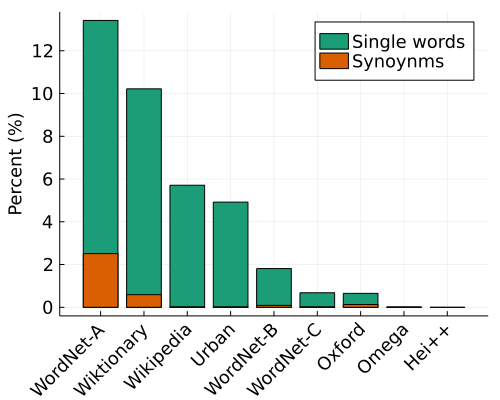
\includegraphics[width=0.7\textwidth]{assets/plots/syn_counts.png}
    \caption{Plot of single word definitions.}
    \label{fig:single_word_defs}
\end{figure}

\FloatBarrier
\section{Challenges and future directions}
Definition modeling faces several challenges, providing new opportunities for future research to be developed.

\noindent\textbf{Polysemes:} The basic definition model cannot be used to generate definitions for \textit{polysemes}, words with multiple definitions. As a
significant challenge for the original definition model, many researchers have
proposed methods to tackle this problem. However, many of the proposed
approaches require the context of the \textit{definiendum} to be provided to the
model. Methods that provide appropriate definitions for polysemes without
context may be valuable in tasks with limited language resources.

\noindent\textbf{Technical terms:} It is challenging to generate definitions for technical terms which require expert knowledge of the field \cite{huang_cdm_2021}. It may
be necessary to provide specific context to generate
definitions for technical terms appropriately. However, obtaining the context requires
scraping and parsing web resources outside of the standard datasets available. Therefore, it may be necessary to generate definitions for technical
terms to augment dictionary datasets properly.

\noindent\textbf{Word combinations:} Complex word combinations, including proverbs and sayings, are rarely covered by sense inventories~\cite{bevilacqua_generationary_2020}. In word combinations, multiple words are used in series to create a new phrase that may be interpreted as a single word for the case of definition modeling. Since the resulting definition
of word combinations may or may not depend on the words used, context may be necessary to parse these word combinations and generate useful definitions. Still, more research is needed to determine if this is the case.
Additionally, word combinations may be absent from the standard dictionary-based datasets.

\noindent\textbf{Non-English words:} As many of the datasets developed for defintion modeling thus far take information from English dictionaries, most methods also
are only applied to English words. In addition, as there exist several lexical resources in other languages, it should be possible to generate definitions for non-English words. To evaluate the quality of word embeddings for
non-English words within definition modeling, it is necessary to develop a method to generate definitions for non-English words. There is some work in Chinese definition modeling \cite{zheng_decompose_2021}, and in French
definition modeling~\cite{reid_vcdm_2020}. However, more research is needed to determine the best method for generating definitions for non-English words, 
especially for a model that can generalize across multiple languages.

\noindent\textbf{Evaluation criteria:} Definition models have been evaluated on a number of metrics, including precision, perplexity, BLEU, and ROUGE. However,
as definition modeling aims to improve the interpretability of word embeddings, it is important to select the evaluation criteria correctly. Many definitions consist of a single word, which can interfere with evaluation metrics such as BLEU and ROUGE scores \cite{mickus_mark_2019}. Human
evaluation of generated definitions can be useful but difficult for researchers to obtain.


\FloatBarrier
\section{Conclusion}
Write text related to conclusion of this study.

\printbibliography
\end{document}
